\documentclass[11pt,a4paper]{article}
\usepackage[utf8]{inputenc}
\usepackage[T1]{fontenc}
\usepackage[british]{babel}
% % Page numbers higher: extra bottom margin; includefoot reserves space for footer
\usepackage[a4paper,left=12mm,right=12mm,top=12mm,bottom=10mm,headheight=5pt,includefoot]{geometry}
\usepackage{booktabs}
\usepackage{array}
\usepackage{makecell}
\usepackage{tabularx}
\usepackage{graphicx}
\usepackage{hyperref}
\usepackage{float}
\usepackage{fancyhdr}
\setcounter{secnumdepth}{-1}

\newcommand{\email}[1]{\texttt{\detokenize{#1}}}
\usepackage{xcolor}   
\usepackage{listings}

\pagestyle{fancy}
\fancyhf{}
\lhead{2026}
\rhead{Predicting The Severity of Traffic Accidents}
\cfoot{\thepage}
\setcounter{secnumdepth}{1}
\setcounter{tocdepth}{1}            
\definecolor{backcolour}{rgb}{0.95,0.95,0.95} 
\definecolor{codegreen}{rgb}{0,0.6,0}         
\definecolor{keywordcolor}{rgb}{0.0, 0.3, 0.7}
\definecolor{stringcolor}{rgb}{0.8, 0.1, 0.1} 

\lstdefinestyle{mycodestyle}{
    backgroundcolor=\color{backcolour},   
    commentstyle=\color{codegreen}\itshape,
    keywordstyle=\color{keywordcolor}\bfseries,
    stringstyle=\color{stringcolor},
    basicstyle=\ttfamily\footnotesize,
    breakatwhitespace=false,         
    breaklines=true,                 
    captionpos=b,                    
    keepspaces=true,                 
    numbers=left,       % Номера строк слева
    numberstyle=\tiny\color{gray},
    numbersep=10pt,                  
    showspaces=false,                
    showstringspaces=false,
    showtabs=false,                  
    tabsize=2,
    frame=single,       % Тонкая рамка вокруг кода
    rulecolor=\color{lightgray}
}
\lstset{style=mycodestyle}

\begin{document}
\begin{titlepage}
  \centering
  \vspace*{2.5cm}
  {\huge\bfseries Predicting The Severity of\\[0.25em]  Traffic Accidents\par}
  \vspace{1.5em}
  {\large Big Data --- Final Project\par}
  \vspace{0.45em}
  {\normalsize Innopolis University\par}
  \vspace{2.8em}
  {\LARGE\bfseries Team 31\par}
  \vspace{2.2em}
  \begin{tabular}{c}
    \textbf{Anna Belyakova} \quad \email{a.belyakova@innopolis.university} \\[0.9em]
    \textbf{Sofia Pushkareva} \quad \email{s.pushkareva@innopolis.university} \\[0.9em]
    \textbf{Daria Alexandrova} \quad \email{d.alexandrova@innopolis.university} \\[0.9em]
    \textbf{Aisylu Fattakhova} \quad \email{a.fattakhova@innopolis.university} \\
  \end{tabular}
  \vfill
  {\large May 9, 2026}
\end{titlepage}

% --- Оглавление ---
\tableofcontents
\newpage

\section{Introduction}
\subsection*{Business objectives}
Traffic accidents pose a significant challenge to public safety, resulting in loss of life, severe injuries, and substantial economic costs due to property damage and traffic congestion. The primary business objective of this project is to develop a robust big data pipeline and a predictive machine learning model capable of classifying the severity of traffic accidents based on real-time features such as weather conditions, time of day, and road environment.

By accurately predicting accident severity immediately upon occurrence using the nationwide US Accidents dataset, several key stakeholders can derive actionable insights:
\begin{itemize}
    \item \textbf{Emergency Medical Services (EMS):} Predicting the potential severity of an incident allows dispatchers to optimize resource allocation, minimizing response times.
    \item \textbf{Department of Transportation (DoT):} Analyzing the correlation between accident severity and various factors helps authorities identify high-risk zones for targeted infrastructure improvements.
    \item \textbf{Navigation Services:} Systems like Google Maps can estimate road clearance times more accurately and proactively reroute drivers.
\end{itemize}

% \section{Data Description}
% \subsection*{Data Characteristics}
% The \href{https://www.kaggle.com/datasets/sobhanmoosavi/us-accidents}{dataset} used in this project is the "US Accidents" dataset, which is a countrywide traffic accident dataset covering 49 states of the United States.

\section{Data Description}

\subsection*{Dataset Overview}
The dataset used in this project is titled \textbf{”US Accidents (2016--2023)”} and was obtained from Kaggle. It is a countrywide traffic accident dataset covering 49 states of the United States. The dataset contains approximately 7.7 million accident records collected from February 2016 to March 2023. The uncompressed CSV file size is massive, requiring distributed big data tools for processing. To ensure efficient processing and balanced analysis, data was chunked and cleaned, and categorical/boolean variables were standardized.

\subsection*{Dataset Source and Purpose}
The original data was collected using multiple APIs that provide streaming traffic incident (or event) data. These APIs broadcast traffic data captured by various entities, including the US and state departments of transportation, law enforcement agencies, traffic cameras, and traffic sensors within the road networks. 

Traffic accidents cause significant economic loss, property damage, and delays. This dataset enables the analysis of environmental, spatial, and temporal factors leading to accidents, providing valuable insights into predictive modeling opportunities for emergency responders and navigation systems.

\subsection*{Dataset Features}
The dataset contains \textbf{46} columns, described as follows:
\begin{enumerate}
    \item \textbf{id:} Unique identifier of the accident record.
    \item \textbf{source:} Source of the accident report (e.g., MapQuest, Bing).
    \item \textbf{severity:} Severity of the accident (target variable, 1 to 4).
    \item \textbf{start\_time:} Start time of the accident in local time zone.
    \item \textbf{end\_time:} End time of the accident in local time zone.
    \item \textbf{start\_lat:} Latitude in GPS coordinates of the start point.
    \item \textbf{start\_lng:} Longitude in GPS coordinates of the start point.
    \item \textbf{end\_lat:} Latitude in GPS coordinates of the end point (if available).
    \item \textbf{end\_lng:} Longitude in GPS coordinates of the end point (if available).
    \item \textbf{distance\_mi:} The length of the road extent affected by the accident in miles.
    \item \textbf{description:} Natural language description of the accident.
    \item \textbf{street:} Street name in the address field.
    \item \textbf{city:} City in the address field.
    \item \textbf{county:} County in the address field.
    \item \textbf{state:} State in the address field.
    \item \textbf{zipcode:} Zipcode in the address field.
    \item \textbf{country:} Country in the address field (US).
    \item \textbf{timezone:} Timezone based on the location of the accident.
    \item \textbf{airport\_code:} Denotes an airport-based weather station closest to the location.
    \item \textbf{weather\_timestamp:} Time-stamp of weather observation record (in local time).
    \item \textbf{temperature\_f:} Temperature (in Fahrenheit).
    \item \textbf{wind\_chill\_f:} Wind chill (in Fahrenheit).
    \item \textbf{humidity\_pct:} Humidity (in percentage).
    \item \textbf{pressure\_in:} Air pressure (in inches).
    \item \textbf{visibility\_mi:} Visibility (in miles).
    \item \textbf{wind\_direction:} Wind direction.
    \item \textbf{wind\_speed\_mph:} Wind speed (in miles per hour).
    \item \textbf{precipitation\_in:} Precipitation amount in inches.
    \item \textbf{weather\_condition:} Weather condition description (e.g., Rain, Snow, Clear).
    \item \textbf{amenity:} Boolean flag indicating presence of an amenity nearby.
    \item \textbf{bump:} Boolean flag indicating presence of a speed bump nearby.
    \item \textbf{crossing:} Boolean flag indicating presence of a crossing nearby.
    \item \textbf{give\_way:} Boolean flag indicating presence of a give-way sign nearby.
    \item \textbf{junction:} Boolean flag indicating presence of a junction nearby.
    \item \textbf{no\_exit:} Boolean flag indicating presence of a no-exit sign nearby.
    \item \textbf{railway:} Boolean flag indicating presence of a railway nearby.
    \item \textbf{roundabout:} Boolean flag indicating presence of a roundabout nearby.
    \item \textbf{station:} Boolean flag indicating presence of a station (e.g., bus, train) nearby.
    \item \textbf{stop:} Boolean flag indicating presence of a stop sign nearby.
    \item \textbf{traffic\_calming:} Boolean flag indicating presence of traffic calming means nearby.
    \item \textbf{traffic\_signal:} Boolean flag indicating presence of a traffic signal nearby.
    \item \textbf{turning\_loop:} Boolean flag indicating presence of a turning loop nearby.
    \item \textbf{sunrise\_sunset:} Indicates day or night based on sunrise/sunset.
    \item \textbf{civil\_twilight:} Indicates day or night based on civil twilight.
    \item \textbf{nautical\_twilight:} Indicates day or night based on nautical twilight.
    \item \textbf{astronomical\_twilight:} Indicates day or night based on astronomical twilight.
\end{enumerate}

\subsection*{Target Variable}
For the purposes of this project, the key variable of interest is \textbf{\texttt{severity}}, which serves as the multi-class label for classification. The goal is to predict this variable based on weather, time, and road characteristics. In this dataset, severity is defined as the impact of the accident on traffic flow, measured on a scale from 1 to 4:
\begin{itemize}
    \item \textbf{1:} Short delay, minimal impact on traffic.
    \item \textbf{2:} Moderate impact, often involving lane closures.
    \item \textbf{3:} High impact, significant traffic congestion.
    \item \textbf{4:} Long-term delay, potentially involving total road closure.
\end{itemize}
\section{Architecture of Data Pipeline}

This project follows an end-to-end Big Data architecture to handle, process, and analyze the large-scale US Accidents dataset. The architecture consists of several well-defined stages, with clear input and output formats at each step:

\begin{enumerate}
    \item \textbf{Data Ingestion (Python $\rightarrow$ PostgreSQL $\rightarrow$ HDFS):}
    \begin{itemize}
        \item \textbf{Input:} Raw CSV file \texttt{US\_Accidents\_March23.csv} (approx. 7.7 million rows).
        \item \textbf{Process:} Processed via Python in chunks of 200,000 rows for deduplication, missing value handling, and coordinate validation. Loaded into PostgreSQL tables using the efficient \texttt{COPY} command. Finally, exported to HDFS using Apache Sqoop.
        \item \textbf{Output:} Files in AVRO format (Snappy-compressed) with accompanying \texttt{.avsc} schema in HDFS.
    \end{itemize}
    \textbf{AVRO} was selected for HDFS storage to ensure robust schema preservation of data types during ingestion and to optimize write performance.
    
    \textbf{Snappy} compression was applied due to its high processing speed and splittability, which facilitates efficient parallel processing across the Hadoop cluster while significantly reducing the disk footprint.

    \item \textbf{Storage and Query (Hive):}
    \begin{itemize}
        \item \textbf{Input:} AVRO files and schema in HDFS.
        \item \textbf{Process:} External tables defined in Hive. To optimize analytical performance, data is then transferred into a final Hive table (\texttt{us\_accidents\_part\_buck}) that is partitioned by \texttt{state} and bucketed by \texttt{severity} into 4 buckets. EDA is performed using HiveQL.
        \item \textbf{Output:} Queryable Hive tables stored in highly compressed ORC format, alongside several exported CSV files containing EDA query results.
    \end{itemize}

    \item \textbf{Analysis and Modeling (PySpark):}
    \begin{itemize}
        \item \textbf{Input:} Optimized Hive ORC tables accessed via Apache Spark.
        \item \textbf{Process:} Advanced feature engineering (including cyclical time transformation and Lat/Lng to ECEF 3D Cartesian coordinates), data scaling, and multi-class classification modeling (Random Forest and Logistic Regression) using Spark MLlib executed on a YARN cluster.
        \item \textbf{Output:} Trained ML models saved to HDFS, along with evaluation metrics and JSON/CSV prediction datasets.
    \end{itemize}

    \item \textbf{Presentation (Dashboard):}
    \begin{itemize}
        \item \textbf{Input:} Analytical EDA results (CSV) and model prediction outputs.
        \item \textbf{Process:} Dashboard design and storytelling to communicate findings.
        \item \textbf{Output:} Interactive dashboard providing visualizations and actionable insights into accident severities.
    \end{itemize}
\end{enumerate}

\section{Data Preparation}

\subsection*{ER Diagram}
The relational model for this project is highly denormalized to optimize analytical queries. It consists of a single primary table \texttt{us\_accidents} where the \texttt{id} column serves as the Primary Key. All temporal, spatial, weather, and road feature attributes are stored as columns within this entity.

\begin{figure}[H]
    \centering
    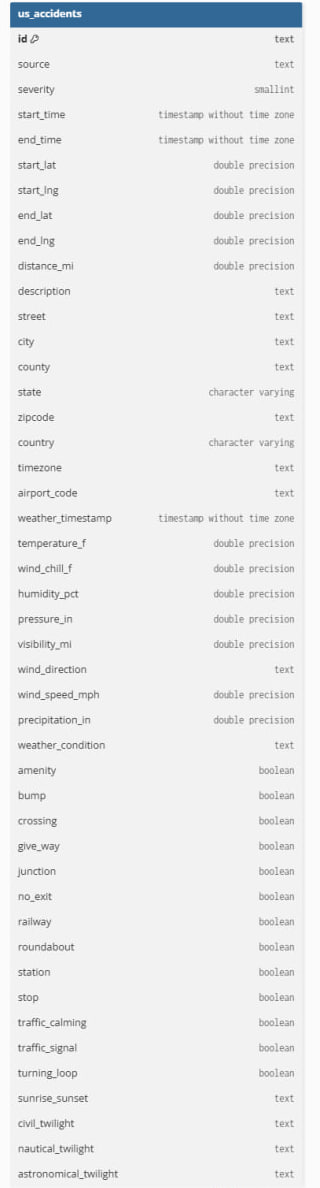
\includegraphics[height=0.85\textheight, keepaspectratio]{er_diagram.jpg} 
    \caption{ER Diagram of the dataset}
\end{figure}


\subsection*{Samples from the database}
After bulk loading the cleaned CSV file using PostgreSQL's \texttt{COPY} command, we verified the integrity of the data. Below is a sample of the structured records.

\begin{figure}[H]
    \centering
    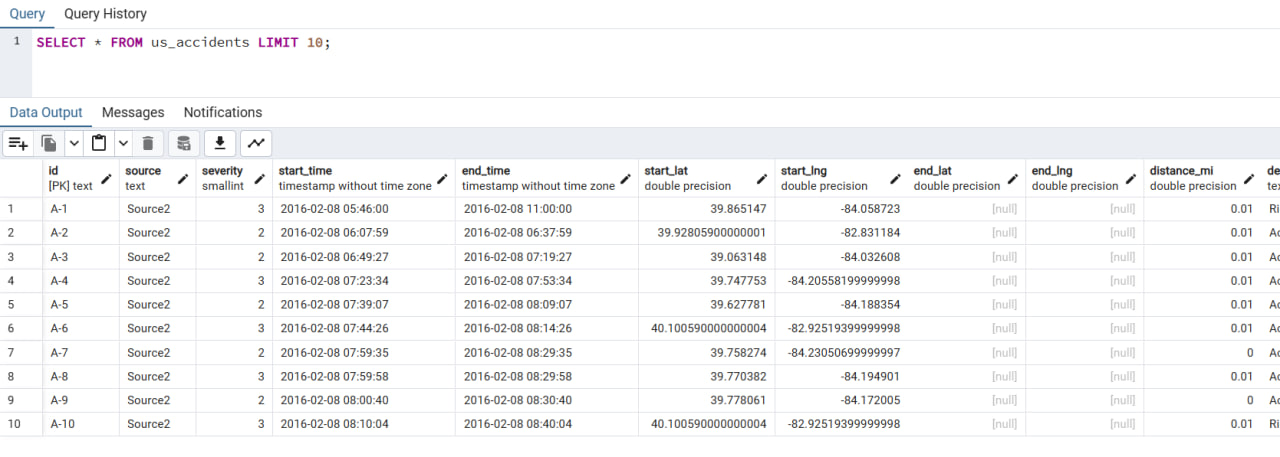
\includegraphics[width=\textwidth]{db_sample.jpg}
    \caption{Sample US Accidents Records from PostgreSQL}
\end{figure}

\subsection*{Data Preparation and Hive Table Creation}
The initial data setup involves preparing HDFS and defining Hive structures. AVRO schemas (\texttt{.avsc} files) generated by Sqoop are first placed in a designated HDFS location. Then, within Hive, the \texttt{team31\_projectdb} database is created. 

To optimize performance, we used a two-step process. First, an external table mapped to the AVRO data was created. Second, the data was inserted into a highly optimized \texttt{us\_accidents\_part\_buck} table, which is partitioned by \texttt{state} and bucketed by \texttt{severity} using the \texttt{ORC} format. Key HiveQL statements for this process include:

\begin{lstlisting}[language=SQL]
CREATE DATABASE IF NOT EXISTS team31_projectdb
  LOCATION 'project/hive/warehouse';

USE team31_projectdb;

-- 1. Create External AVRO Table
CREATE EXTERNAL TABLE IF NOT EXISTS us_accidents
  STORED AS AVRO
  LOCATION 'project/warehouse/us_accidents'
  TBLPROPERTIES ('avro.schema.url'='project/warehouse/avsc/us_accidents.avsc');

-- 2. Create Optimized ORC Table (Partitioned & Bucketed)
CREATE EXTERNAL TABLE IF NOT EXISTS us_accidents_part_buck (
  id STRING, source STRING, severity INT, start_time TIMESTAMP, 
  -- [other columns omitted for brevity] --
  astronomical_twilight STRING
)
PARTITIONED BY (state STRING)
CLUSTERED BY (severity) INTO 4 BUCKETS
STORED AS ORC
LOCATION 'project/hive/warehouse/us_accidents_part_buck'
TBLPROPERTIES ('orc.compress'='NONE');
\end{lstlisting}

\subsection*{Script Execution Workflow}
The entire data ingestion and processing pipeline is orchestrated via bash scripts. These scripts handle Sqoop imports, upload AVRO schemas to HDFS, and execute a sequence of HiveQL scripts using \texttt{beeline}. Example commands from our execution workflow are:

\begin{lstlisting}[language=bash]
# Uploading AVSC schema file to HDFS
hdfs dfs -mkdir -p "project/warehouse/avsc"
hdfs dfs -put "output/sqoop_generated/us_accidents.avsc" \
              "project/warehouse/avsc/us_accidents.avsc"

# Executing HiveQL scripts via Beeline
beeline -u "jdbc:hive2://hadoop-03.uni.innopolis.ru:10001" -n "team31" \
  -p "$HIVE_PASSWORD" --hiveconf "DB_NAME=team31_projectdb" \
  -f hive/create_external_table.hql
\end{lstlisting}
\section{Data Analysis}

Exploratory Data Analysis (EDA) was performed using HiveQL. The queries aggregated the 7.7 million records across multiple dimensions including time, location, weather, and road infrastructure. The key findings were visualized to identify patterns that lead to traffic accidents and to understand the distribution of our target variable.

\subsection*{Analysis Results. Main insights}

\begin{itemize}
    \item \textbf{Target Variable Imbalance (Severity Distribution)}
    
    The analysis of the \texttt{severity} column reveals a massive class imbalance in the dataset. Nearly 80\% (79.67\%) of all accidents are classified as Severity 2 (moderate impact, such as a lane closure). Severity 3 accounts for 16.81\%, while extreme cases—Severity 4 (total road closure) and Severity 1 (minimal impact)—make up only 2.65\% and 0.87\% respectively. This baseline metric is crucial as it dictates the necessity of using the F1-score rather than raw accuracy during the Machine Learning evaluation phase.

    \begin{figure}[H]
        \centering
        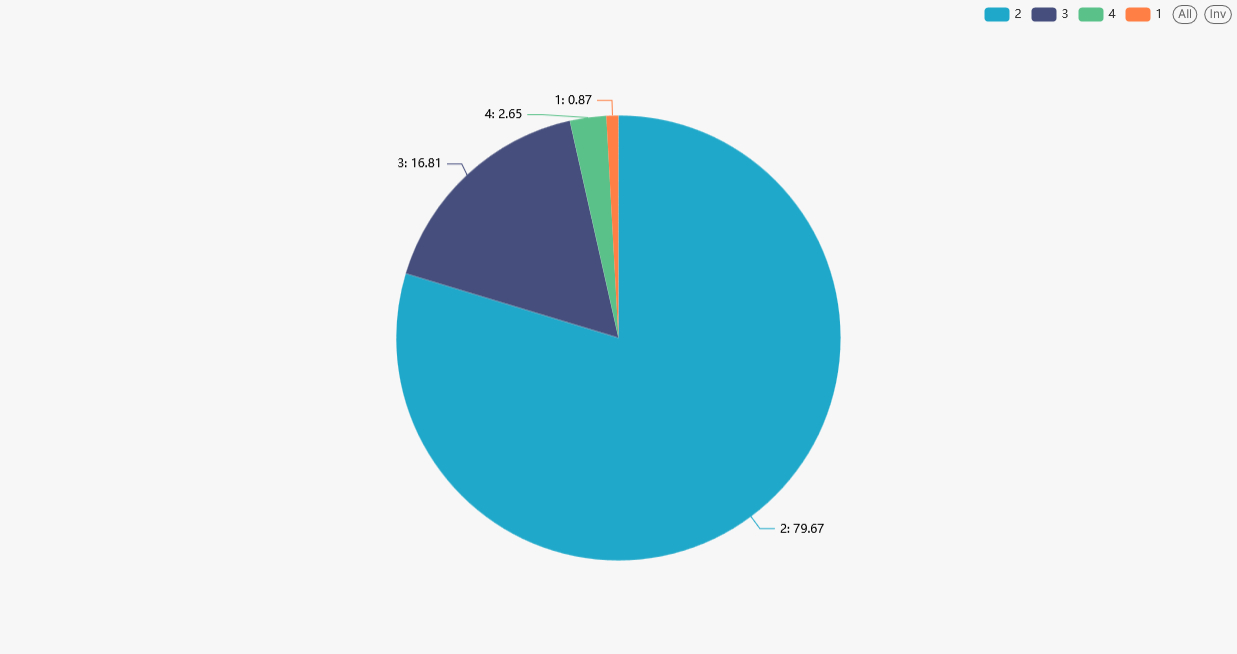
\includegraphics[width=0.8\textwidth]{q7.jpg}
        \caption{Insight 1: Overall Accident Severity Distribution}
    \end{figure}

    \item \textbf{Temporal Patterns (Accidents by Hour of Day)}
    
    The data shows a clear, classic bi-modal distribution corresponding to daily commuting patterns. Accidents peak sharply during the morning rush hour (7:00 AM -- 9:00 AM), reaching up to 587k incidents at 7:00 AM. A second, equally massive peak occurs during the evening commute (4:00 PM -- 6:00 PM), peaking at 582k incidents at 5:00 PM. This confirms that traffic volume is the absolute primary driver of accident frequency.

    \begin{figure}[H]
        \centering
        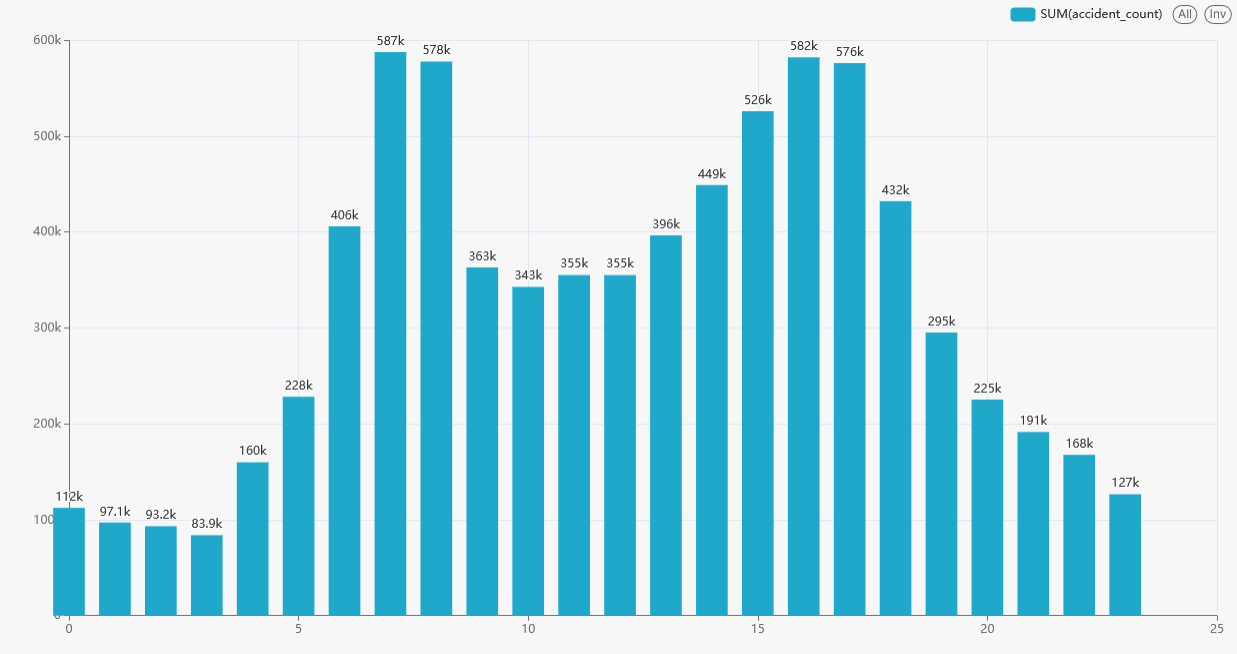
\includegraphics[width=\textwidth]{q5.jpg}
        \caption{Insight 2: Accident Frequency by Hour of the Day}
    \end{figure}

    \item \textbf{Impact of Road Features}
    
    Analyzing boolean road features reveals where accidents are most likely to occur in relation to infrastructure. Junctions (20.23\%) and Give Way signs (12.20\%) are associated with the highest number of infrastructure-related accidents. This aligns with traffic dynamics, as junctions require lane changes, merging, and crossing traffic flows, inherently increasing collision risks. Conversely, Roundabouts account for only 3.34\%, suggesting they might be a safer intersection design.

    \begin{figure}[H]
        \centering
        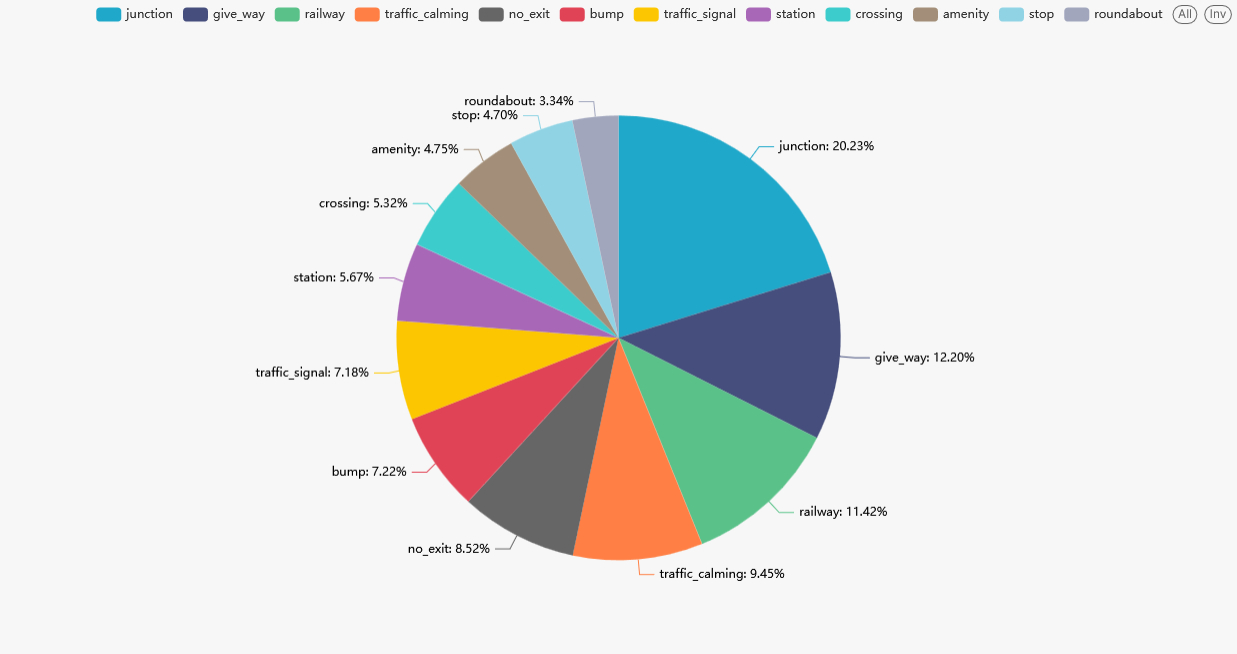
\includegraphics[width=0.9\textwidth]{q1.jpg}
        \caption{Insight 3: Proportion of Accidents Near Specific Road Features}
    \end{figure}

    \item \textbf{Geographical Hotspots (Top Cities)}
    
    When grouping accidents by city, Miami leads significantly with 187k recorded accidents, followed by Houston (169k) and Los Angeles (156k). These cities are characterized by massive urban sprawl, high population density, and heavy reliance on personal vehicles and highway networks, making them prime hotspots for traffic incidents.

    \begin{figure}[H]
        \centering
        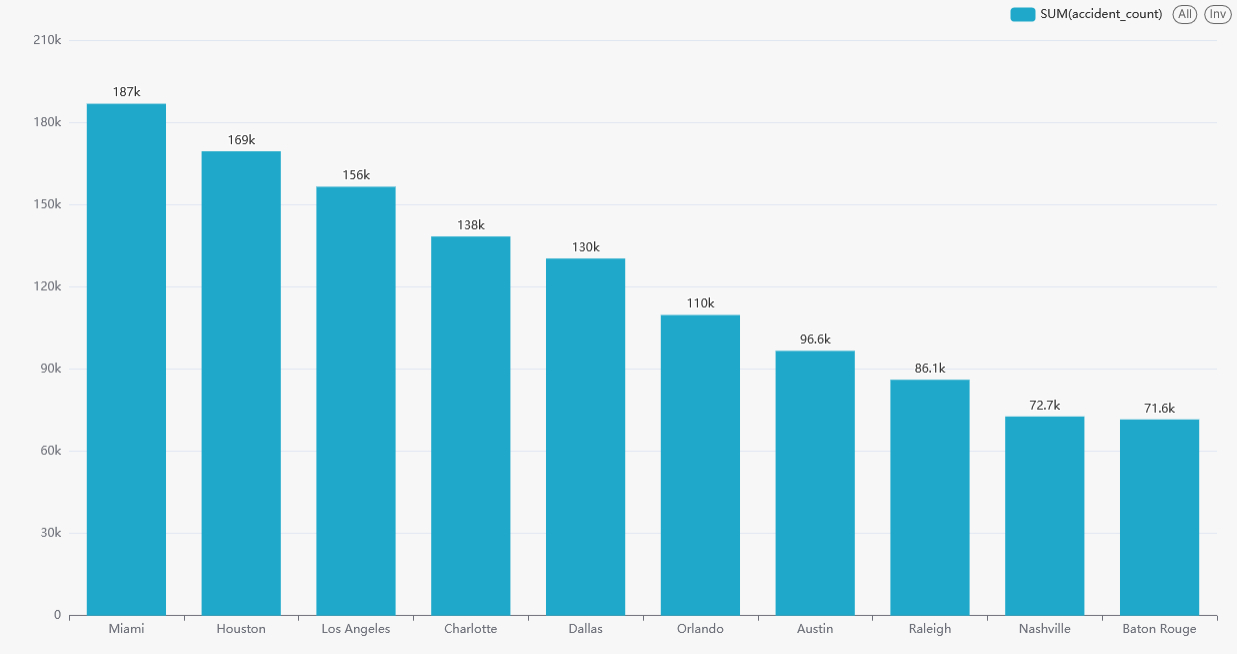
\includegraphics[width=\textwidth]{q4.jpg}
        \caption{Insight 4: Top 10 Cities with Highest Accident Counts}
    \end{figure}

    

    \item \textbf{Weather Conditions Overview}
    
    The analysis of weather conditions indicates a wide diversity of atmospheric states during accidents. While many accidents happen under clear or mostly cloudy skies (simply because these are the most common weather states), a significant portion of incidents is distributed across adverse conditions like Scattered Clouds, Overcast, Rain, and Snow. 

    \begin{figure}[H]
        \centering
        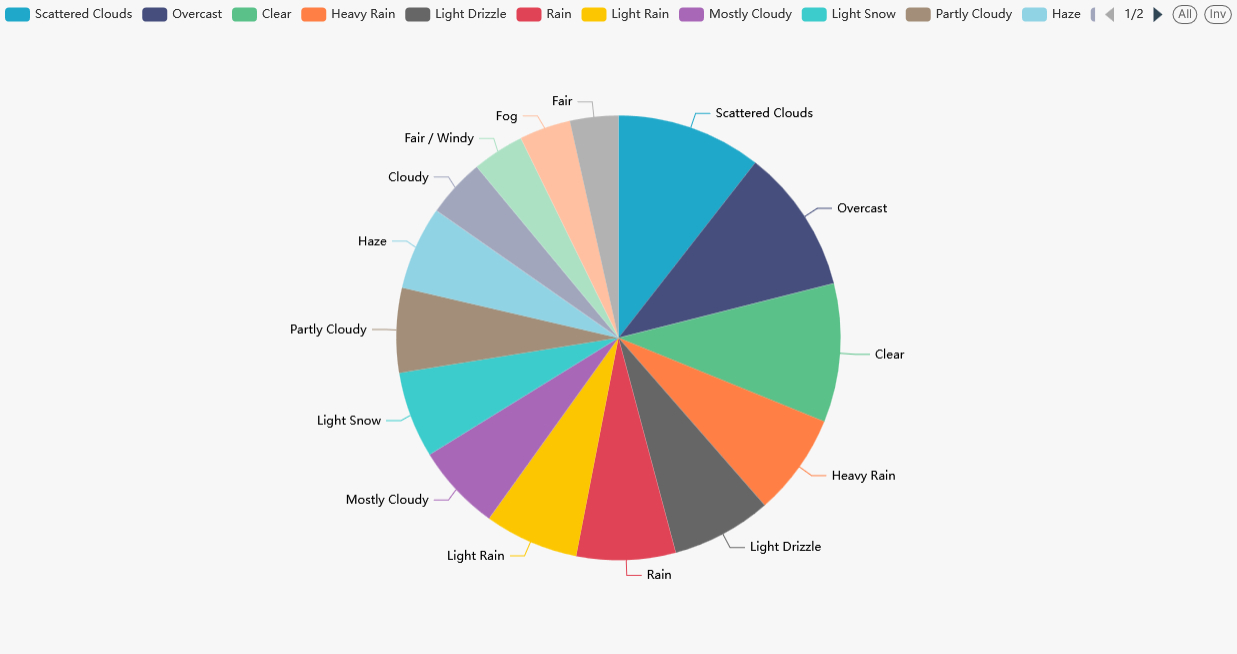
\includegraphics[width=0.9\textwidth]{q6.jpg}
        \caption{Insight 5: Diversity of Weather Conditions During Accidents}
    \end{figure}

    \item \textbf{The Paradox of Visibility and Wind Speed on Severity}
    
    An intriguing insight emerges when correlating high-severity accidents (Severity 3 and 4) with visibility and wind speed:
    \begin{itemize}
        \item \textbf{Visibility:} High severity peaks at moderate visibility (1-7 miles) at $\sim$21\%. Surprisingly, near-zero visibility (0-1 miles) has the lowest high-severity rate (17.58\%). 
        \item \textbf{Wind Speed:} Similarly, high severity peaks during moderate-to-strong winds (15-35 mph). At extreme wind speeds (35+ mph), the severity rate drops to 18.03\%.
    \end{itemize}
    \textit{Interpretation:} This counter-intuitive trend suggests a behavioral shift. In absolutely extreme conditions (zero visibility, hurricane winds), drivers either stay home or drive extremely slowly, resulting in minor fender-benders. In moderate-to-bad conditions, drivers often maintain highway speeds, leading to much more severe impacts when collisions occur.

    \begin{figure}[H]
        \centering
        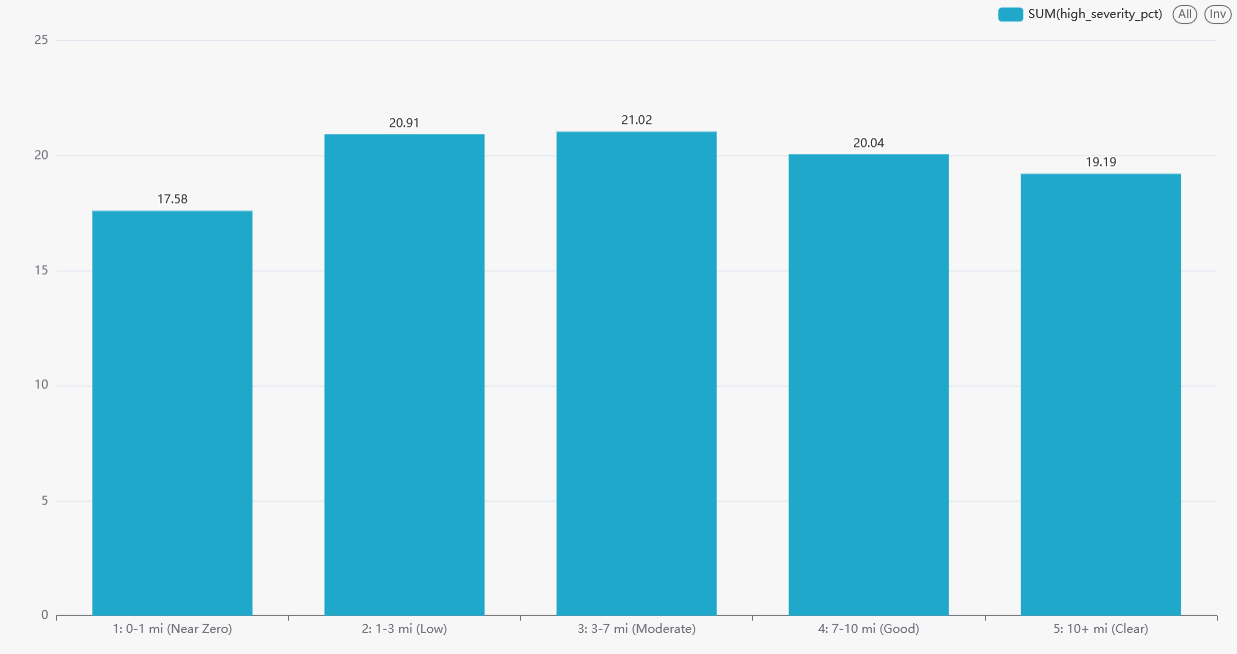
\includegraphics[width=\textwidth]{q3.jpg}
        \caption{Insight 6: Percentage of High Severity Accidents by Visibility Range}
    \end{figure}

    \begin{figure}[H]
        \centering
        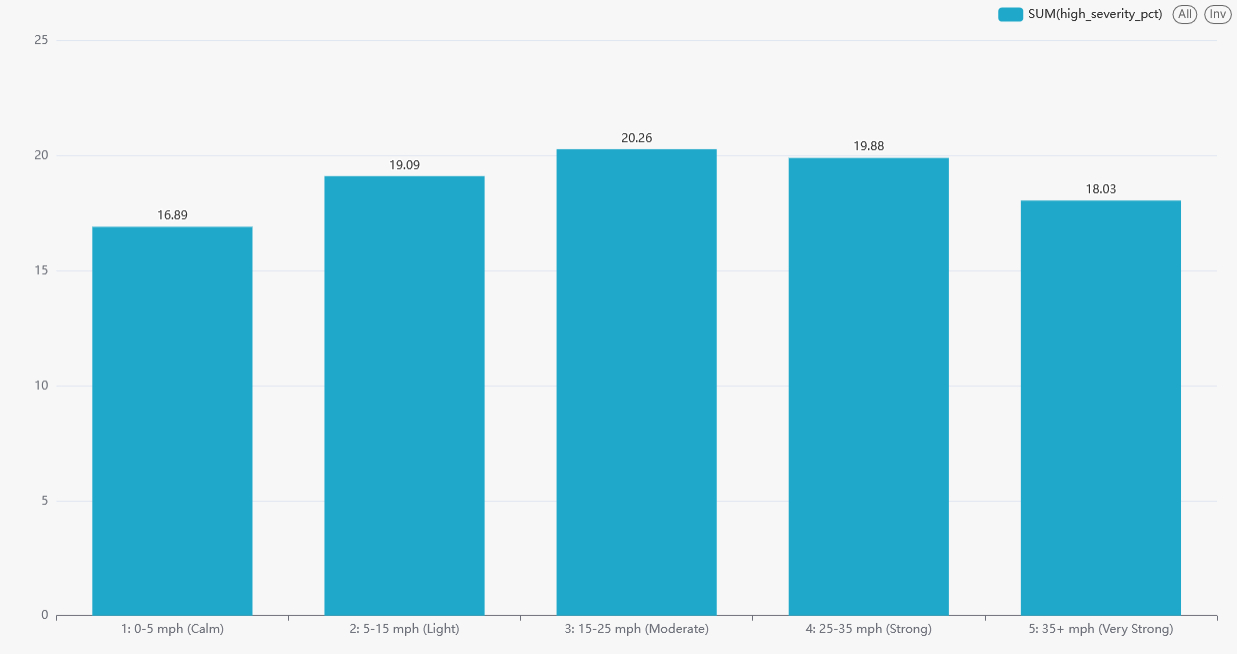
\includegraphics[width=\textwidth]{q2.jpg}
        \caption{Insight 7: Percentage of High Severity Accidents by Wind Speed Range}
    \end{figure}

\end{itemize}
\section{Modeling and Prediction}

The primary objective of this stage was to develop, train, and evaluate machine learning models using PySpark MLlib to predict the severity of traffic accidents. The process involved comprehensive data preparation, advanced feature engineering, model selection, hyperparameter tuning, and evaluation, all executed on a distributed YARN cluster leveraging data stored in Hive and HDFS.

\subsection*{Dataset overview}
\begin{itemize}
    \item \textbf{Source:} Data was extracted from the \texttt{team31\_projectdb} database, from an optimized Hive table named \texttt{us\_accidents\_part\_buck}.
    \item \textbf{Target variable:} The multi-class column \texttt{severity} (values 1 to 4). For Spark ML compatibility, this was shifted to a 0-to-3 index (\texttt{label = severity - 1.0}).
    \item \textbf{Initial size:} The raw dataset contained \textbf{7,728,394 records}.
\end{itemize}

\subsection*{Data preparation pipeline}
A robust preprocessing pipeline was constructed using PySpark to prepare the data for multi-class classification modeling:

\begin{enumerate}
    \item \textbf{Feature selection and missing values handling:} 
    A total of \textbf{41 features} were selected, including temporal, environmental, and road infrastructure variables. Rows with null values in essential columns (\texttt{severity}, \texttt{start\_time}, \texttt{start\_lat}, \texttt{start\_lng}) were filtered out. For other columns, missing categorical values were replaced with \texttt{"unknown"}, missing numericals with \texttt{0.0}, and missing booleans with \texttt{False}.
    
    \item \textbf{Advanced Time features decomposition:} 
    Raw timestamps were replaced by a custom transformer called \texttt{CyclicalTimestampTransformer}. Temporal components (month, day, hour) were transformed using sine and cosine functions to accurately capture their cyclical nature (e.g., ensuring 23:00 and 01:00 are recognized as being close in time).
    
    \item \textbf{Geospatial transformation:} 
    A custom \texttt{LatLngToEcefTransformer} converted raw GPS coordinates (Latitude/Longitude) into 3D Cartesian coordinates (\texttt{ecef\_x, ecef\_y, ecef\_z}) to provide a better spatial representation for the decision trees.
    
    \item \textbf{Categorical features encoding:} 
    String features such as \texttt{state}, \texttt{wind\_direction}, and \texttt{weather\_condition} were converted into numerical indices using \texttt{StringIndexer}.
    
    \item \textbf{Feature assembling and scaling:} 
    All 41 processed features (booleans, cyclical time, ECEF coordinates, scaled numericals, and indexed categoricals) were combined into a single feature vector column using \texttt{VectorAssembler}. The assembled vector was then standardized using \texttt{StandardScaler}.
    
    \item \textbf{Train-test split:} 
    The dataset was randomly split into training (60\%) and testing (40\%) sets using a fixed seed for reproducibility.
\end{enumerate}

\subsection*{ML model training with hyperparameters tuning}
Two classification models were trained and tuned using 3-fold cross-validation on the training data. The \texttt{MulticlassClassificationEvaluator} with the weighted F1-score metric was used to guide hyperparameter selection, which is critical due to the massive class imbalance (Severity 2 dominating).

\begin{itemize}
    \item \textbf{Multinomial Logistic Regression}
    \begin{itemize}
        \item Hyperparameters tuned via ParamGrid: \texttt{regParam} ($[10^{-3}, 10^{-2}, 0.05]$), \texttt{elasticNetParam} ($[0.0, 0.5]$).
    \end{itemize}
    \item \textbf{Random Forest Classifier}
    \begin{itemize}
        \item Hyperparameters tuned via ParamGrid: \texttt{numTrees} ($[40, 80, 120]$), \texttt{maxDepth} ($[6, 10]$).
        \item Best parameters found: \texttt{numTrees = 40}.
    \end{itemize}
\end{itemize}

\subsection*{Model evaluation and comparison}
Models were evaluated on the 40\% test set using Accuracy and the weighted F1-score. 

\begin{table}[H]
    \centering
    \renewcommand{\arraystretch}{1.3}
    \begin{tabular}{|l|c|c|c|c|}
        \hline
        \textbf{Model} & \textbf{numClasses} & \textbf{numFeatures} & \textbf{Accuracy} & \textbf{F1-score} \\
        \hline
        Logistic Regression & 4 & 41 & 79.95\% & 76.19\% \\
        \hline
        \textbf{Random Forest} & \textbf{4} & \textbf{41} & \textbf{81.86\%} & \textbf{76.72\%} \\
        \hline
    \end{tabular}
    \caption{Model Comparison Metrics on Test Set}
\end{table}

As shown in Table 1, the Random Forest classifier demonstrated superior performance across all evaluated metrics. It successfully captured the non-linear relationships between weather conditions, road infrastructure, and time, achieving the highest Accuracy (81.86\%) and F1-score (76.72\%).

\subsection*{Model and prediction outputs}
\begin{itemize}
    \item \textbf{Models saved:} The best trained Logistic Regression and Random Forest models were serialized and saved to HDFS (in the \texttt{project/models/} directory).
    \item \textbf{Predictions saved:} Predictions made by both models on the test set, containing the actual \texttt{label} and the \texttt{prediction}, were saved to HDFS as JSON and CSV files.
    \item \textbf{Evaluation results saved:} The comparison metrics were saved to HDFS as \texttt{evaluation.csv} for integration into the final visualization dashboard.
\end{itemize}
\section{Data presentation}
To present our findings, we developed a multi-tab interactive dashboard in Apache Superset. The dashboard is publicly available at \href{}{link}.

\noindent It consists of three main tabs:

\subsection*{Tab 1: Data Description}
This tab provides a high-level summary of the raw data characteristics.
\begin{itemize}
    \item \textbf{Big Number Indicators:} Showcases the 7.7M records, 46 features, and 49 states coverage.
    \item \textbf{Data Dictionary:} Explains the datatypes (Double, String, Boolean) and the Stage 1 cleaning process.
    \item \textbf{Dataset Sample:} A live table previewing the first 10 records.
\end{itemize}
\begin{figure}[H]
    \centering
    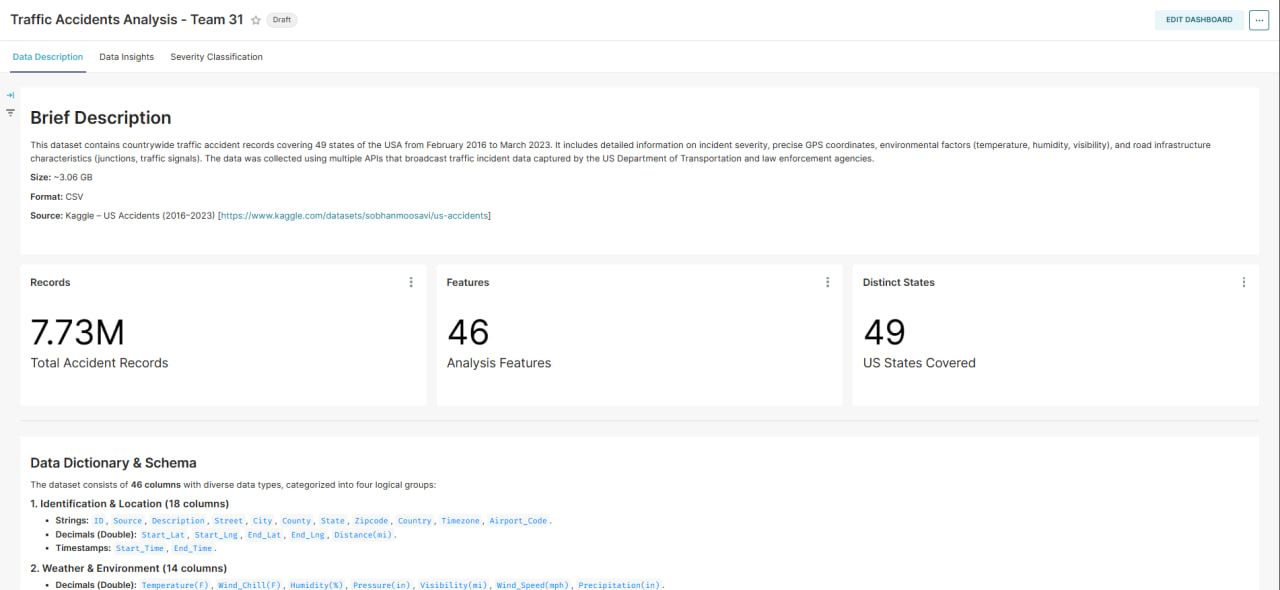
\includegraphics[width=\textwidth]{tab1.jpg}
    \caption{Dashboard Tab 1 -- Data Overview}
\end{figure}

\subsection*{Tab 2: Data Insights (EDA)}
Includes seven visual charts supporting the exploratory data analysis, such as overall accident severity distribution, hourly frequency trends, geographical hotspots by city, and the correlation between incident severity and environmental factors like visibility, wind speed, and road infrastructure characteristics. Each insight is also documented and interpreted in detail in Data Analysis Section of the report.

\begin{figure}[H]
    \centering
    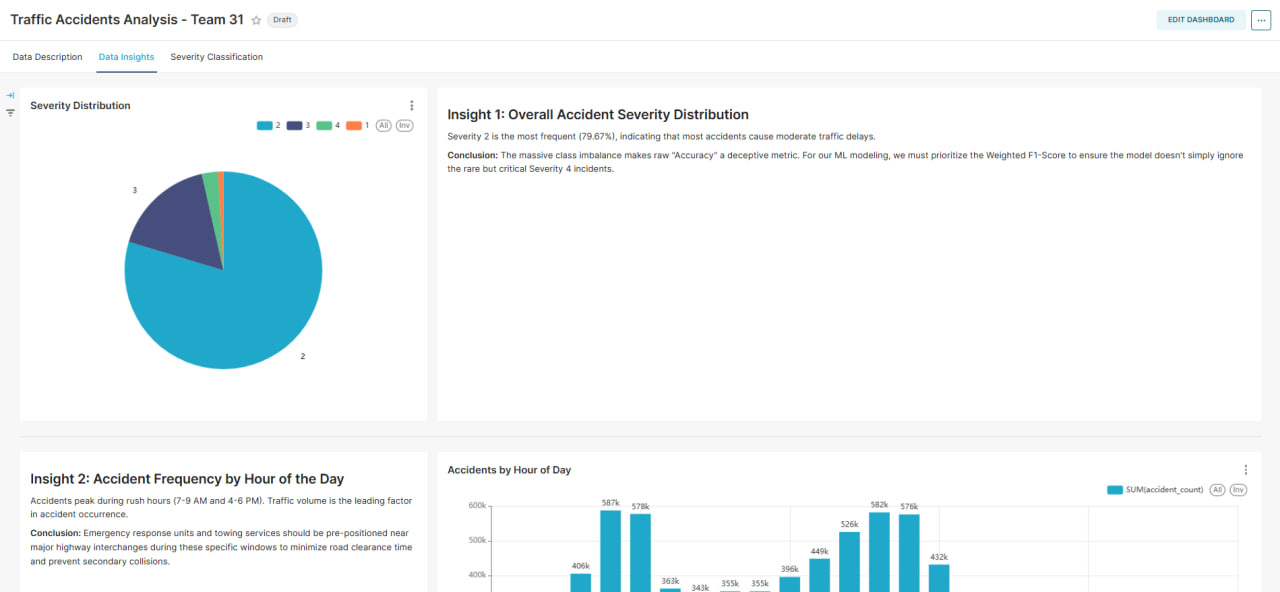
\includegraphics[width=\textwidth]{tab2.jpg}
    \caption{Dashboard Tab 2 -- Exploratory Data Analysis}
\end{figure}

\subsection*{Tab 3: Severity Prediction}
This tab presents the final stage of the project — model evaluation and multi-class prediction of accident severity. It includes:

\begin{itemize}
    \item \textbf{Overview panel:} Summarizes the goal of building a multi-class classifier using PySpark MLlib to predict the target variable \texttt{severity}. It highlights the dataset distribution of approximately 7.7 million records, noting the significant class imbalance where Severity 2 accounts for 79.67\% of all incidents.
    
    \item \textbf{Model training summary:} Outlines the distributed training and hyperparameter tuning process performed on the YARN cluster. For each model, the grid search configuration and the best selected parameters are listed (e.g., \texttt{regParam = 0.01} and \texttt{elasticNetParam = 0.0} for Logistic Regression; \texttt{numTrees = 40} and \texttt{maxDepth = 10} for Random Forest).
    
    \item \textbf{Performance metrics:} Evaluation results for the best models are displayed using Accuracy and Weighted F1-score. As detailed in the ML Modeling section, the Random Forest model achieved the highest performance with an accuracy of 81.86\% and an F1-score of 76.72\%, consistently outperforming the Logistic Regression baseline.
    
    \item \textbf{Prediction examples:} Two interactive tables visualize live prediction samples from the test set. These tables compare the \texttt{Actual} labels versus the \texttt{Predicted} severity levels (indexed 0--3), allowing users to observe the model's classification tendencies.
\end{itemize}
\begin{figure}[H]
    \centering
    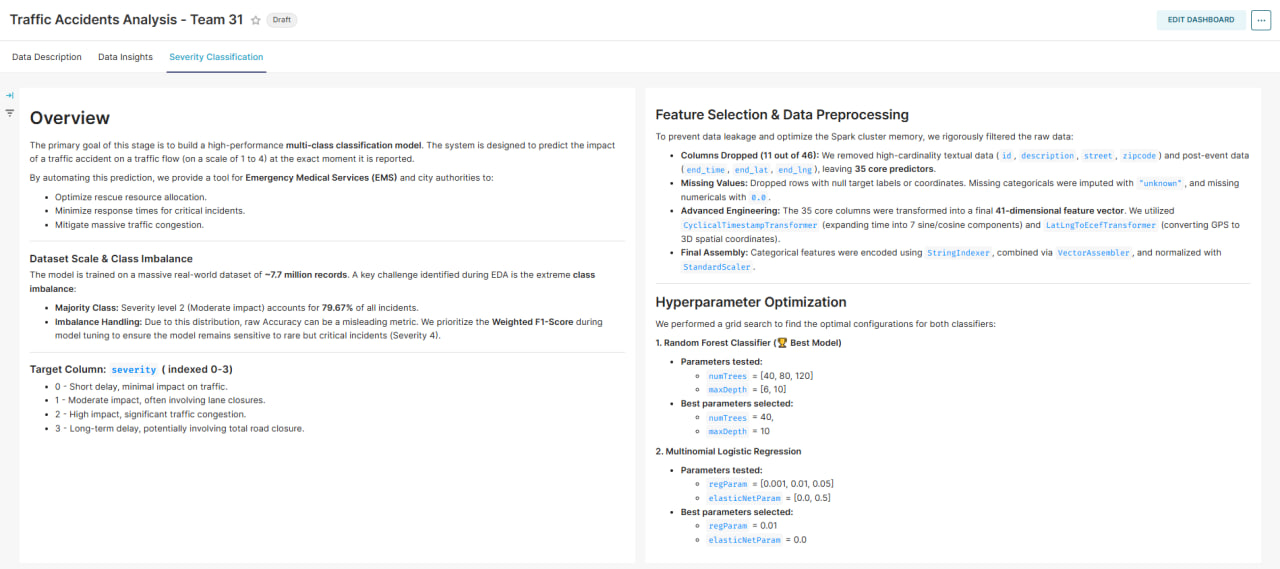
\includegraphics[width=\textwidth]{tab3.jpg}
    \caption{Model overview and training settings}
\end{figure}
\begin{figure}[H]
    \centering
    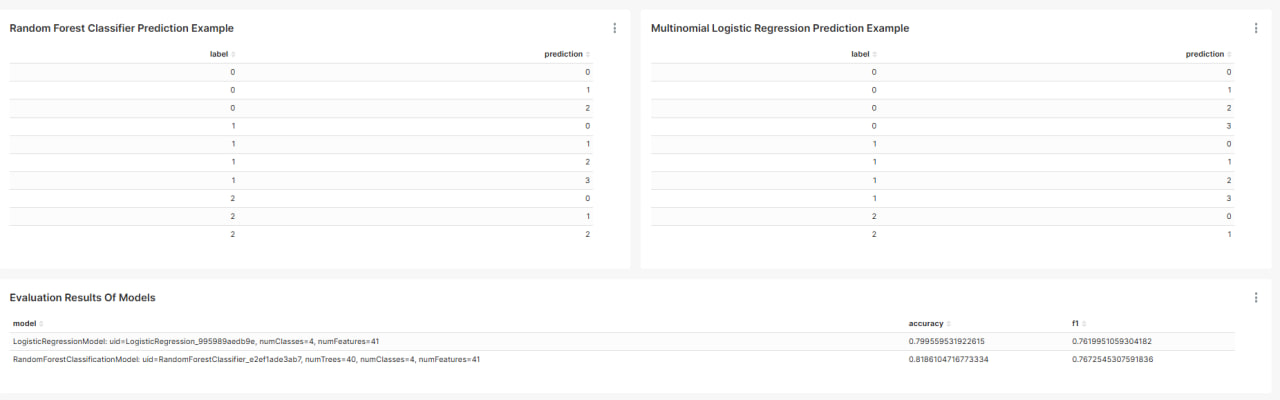
\includegraphics[width=\textwidth]{tab3_1.jpg}
    \caption{Evaluation results and example predictions for both models
}
\end{figure}
\subsection*{Findings}
The most critical finding is that accident severity is not entirely random; it is highly correlated with geographical location (ECEF coordinates) and specific temporal periods. While road features like traffic signals reduce minor accidents, severe accidents (Level 3 and 4) are heavily influenced by a combination of high-speed roads and sudden drops in visibility or adverse weather.

\section{Conclusion}
\subsection*{Summary of the report}
In this project, we successfully developed and deployed an end-to-end Big Data pipeline for predicting traffic accident severity. The key achievements include:
\begin{itemize}
    \item Successfully handled a massive dataset of 7.7 million records, implementing a robust ETL process from raw CSV to a distributed Hadoop ecosystem.
    \item Leveraged PostgreSQL for initial staging and Apache Hive for optimized analytical warehousing.
    \item Utilized Apache Spark MLlib to build a predictive pipeline incorporating custom transformations.
    \item Developed a Random Forest classifier that achieved an accuracy of 81.86\% and F1-Score 76.72\%.
    \item Built Apache Superset dashboard.
\end{itemize}

\section{Reflections on own work}
\subsection*{Challenges and difficulties}
During the development process, we faced several difficulties:
\begin{itemize}
    \item Memory Management
    \item Data Imbalance
    \item Working in cluster in the first time
    \item Superset is not intuitively understandable
    \item Cluster is down several times
\end{itemize}

\subsection*{Recommendations}
For future iterations of this project, we recommend the following enhancements:
\begin{itemize}
    \item \textbf{Real-Time Ingestion:} Integrate Apache Kafka to allow the model to ingest streaming traffic data and provide instantaneous severity predictions.
    \item \textbf{Imbalance Mitigation:} Implement advanced techniques such as SMOTE or class-weighting within Spark to improve the recall of critical Severity 4 accidents.
    \item \textbf{Feature Expansion:} Incorporate external data sources such as high-resolution road surface sensors and real-time traffic flow density to increase predictive precision.
\end{itemize}

\section*{The table of contributions of each team member}
\addcontentsline{toc}{section}{The table of contributions of each team member}

\vspace{0.8em}
\scriptsize % Используем мелкий шрифт, чтобы всё влезло
\setlength{\tabcolsep}{2pt} % Максимально сужаем отступы между колонками
\renewcommand{\arraystretch}{1.5}

\noindent
\begin{tabularx}{\linewidth}{@{} >{\raggedright\arraybackslash}p{2cm} >{\raggedright\arraybackslash}X cccc >{\raggedright\arraybackslash}X c @{}}
  \toprule
  \makecell{\textbf{Project}\\\textbf{tasks}}
    & \textbf{Task description}
    & \makecell{\textbf{Anna}\\\textbf{B.}}
    & \makecell{\textbf{Daria}\\\textbf{A.}}
    & \makecell{\textbf{Sofia}\\\textbf{P.}}
    & \makecell{\textbf{Aisylu}\\\textbf{F.}}
    & \textbf{Deliverables}
    & \makecell{\textbf{Hrs}} \\
  \midrule
  \textbf{Stage I:} Ingestion
    & Data collection (Kaggle API), Python chunked cleaning, and Sqoop import to HDFS.
    & 100\% & 0\% & 0\% & 0\%
    & \texttt{preprocess\_data.py}, \texttt{import\_to\_hdfs.sh}, \texttt{stage1.sh}, \texttt{build\_projectdb.py}, \texttt{data\_collection.sh}, \texttt{data\_storage.sh},
    \texttt{preprocess.sh}, \texttt{sql/*.sql}
    & 12 \\
  \textbf{Stage II:} Storage
    & Hive warehouse design, partitioning by state, bucketing, and HiveQL analytics (Q1--Q7).
    & 0\% & 100\% & 0\% & 0\%
    & \texttt{stage2.sh}, \texttt{hive/*.hql}, \texttt{output/q*.csv}
    & 14 \\
  \textbf{Stage III:} Spark ML
    & Distributed ML pipeline, ECEF/Cyclical features, Random Forest/LR training.
    & 0\% & 0\% & 100\% & 0\%
    & \texttt{train\_ml.py}, \texttt{models/}, \texttt{evaluation.csv}, \texttt{stage3.sh}
    & 18 \\
  \textbf{Stage IV:} Presentation
    & Superset Dashboard design, storytelling, and Tab 1--3 visual insights.
    & 0\% & 0\% & 0\% & 100\%
    & Published Dashboard, Tab screenshots
    & 10 \\
  \textbf{Automation}
    & Development of \texttt{stage4.sh} for integration between Spark and Superset.
    & 0\% & 0\% & 0\% & 100\%
    & \texttt{stage4.sh}, \texttt{report/}
    & 4 \\
  \textbf{Reporting}
    & Technical documentation, LaTeX formatting, and pipeline summary.
    & 0\% & 0\% & 0\% & 100\%
    & \texttt{report.pdf}
    & 15 \\
  \bottomrule
\end{tabularx}
\normalsize

\section{References}
\begin{itemize}
    \item \href{https://github.com/Big-Data-IU/US-Accidents}{Our Github Repository}
    \item \href{https://www.kaggle.com/datasets/sobhanmoosavi/us-accidents}{Kaggle Dataset: US Accidents (2016 - 2023)}
\end{itemize}

\end{document}